\documentclass[landscape,a0]{a0poster_csml_v2}
% NOTE: to remove logo from title, just use \headerNoLogo option below
% Options (don't put spaces between options!)
% portrait and landscape: format of the page 
% A0, A1, A2, A3, A4 : size of the poster

% compared to the old mpi poster style, two things have changed: 
% - it now can be compiled with both (ps)latex and pdflatex
% - there are different variants for headers: one with the mpi logos, 
%   and one where you can include arbitrary files as logos (or have no
%   logos at all). 
% 


% if you want to use pdflatex, then include the commands:
\usepackage[pdftex]{graphicx}
\DeclareGraphicsExtensions{.pdf}
% if you want to use (ps)latex, then include the commands: 
%\usepackage{graphics}
%\DeclareGraphicsExtensions{.eps}
\usepackage[usenames,dvipsnames]{color}

\usepackage{amssymb,amsmath,bbold}

%\usepackage[utf8]{inputenc}
%\usepackage[T1]{fontenc}
%\usepackage{verbatim}
%\usepackage{caption}
%custom packages
\usepackage{amssymb,amsmath}




\usepackage{relsize}

\definecolor{g}{rgb}{0.3,0.61,0.59}


\newcommand\independent{\protect\mathpalette{\protect\independenT}{\perp}}
\def\independenT#1#2{\mathrel{\rlap{$#1#2$}\mkern2mu{#1#2}}}
\newcommand{\trans}{^{\scriptscriptstyle \top}}


\newcommand{\ev}{\mathcal{E}}
\newtheorem{theorem}{Theorem}

% size of the columns of the poster, relative to the width of the
% whole poster: 
\renewcommand{\columnfrac}{.3}% i.e. want three columns
\newcommand{\half}{\frac{1}{2}}



%Kenji macros
\newcommand{\hS}{\widehat{C}} %empirical covariance
\newcommand{\pS}{C} %population covariance
\newcommand{\hlam}{\widehat{\lambda}}
\newcommand{\lam}{\lambda}



\usepackage{natbib}

\usepackage{enumitem}


\begin{document}
\begin{poster}

%------------------------------------------------------------
% header: 
%------------------------------------------------------------

% Additionally to the 'normal' font size commands as
% \tiny,\small,\large\ (look them up in a latex book) there are now
% the fonts \veryHuge, \VeryHuge, \VERYHuge

%title: 
\savebox{\PosterTitle}{\VeryHuge A Wild Bootstrap for Degenerate Kernel Tests}
%authors:
\savebox{\PosterAuthor}{\Large 
Kacper Chwialkowski$^2$, Dino Sejdinovic,$^1$ ,Arthur Gretton,$^1$}
%addresses:
\savebox{\PosterAddress}{\large 
$^1$Gatsby Unit, CSML, UCL, UK; and $^2$CS, UCL, UK;}

% Logos: 

% you can either use the standard MPI header 
% (make sure the logo files logo_mpi.pdf and logo_kyb.pdf are in your
% latex path):
\headerMpi 


% the new color can then be used with the command \color{name}
%\definecolor{anewcolor}{rgb}{0.5,0,0}
%\newcommand{\ulescolor}{\bf \color{anewcolor}}
\definecolor{mpigreen}{rgb}{0.3,0.61,0.59}
\definecolor{mpigrey}{rgb}{0.86,0.85,0.83}
\definecolor{red}{rgb}{1,0,0}
\definecolor{brightgreen}{rgb}{0,1,0}
\definecolor{palepink}{rgb}{1.0,0.4,0.4}
\definecolor{anublue}{rgb}{0,0.5,0.9}
\definecolor{blue}{rgb}{0,0,1}
\definecolor{engPink}{cmyk}{0.0,0.4,0.44,0.33}

\definecolor{1}{rgb}{ 0.9000,0.4909,0}
\definecolor{2}{rgb}{ 0.8182 ,   0.9000,         0}
\definecolor{3}{rgb}{ 0.3273,    0.9000    ,     0}
\definecolor{4}{rgb}{    0  ,  0.9000 ,   0.1636}
\definecolor{5}{rgb}{   0  ,  0.9000  ,  0.6545}
\definecolor{6}{rgb}{   0  ,  0.6545   , 0.9000}
\definecolor{7}{rgb}{  0  ,  0.1636 ,   0.9000}
\definecolor{8}{rgb}{ 0.3273  ,       0  ,  0.9000}
\definecolor{9}{rgb}{ 0.8182  ,       0  ,  0.9000}
\definecolor{10}{rgb}{  0.9000  ,       0  ,  0.4909}


\newcommand{\Mpigreen}[1]{\color{mpigreen}{#1}\color{black}}
\newcommand{\Mpigrey}[1]{\color{mpigrey}{#1}\color{black}}
\newcommand{\Red}[1]{\color{red}{#1}\color{black}}
\newcommand{\Brightgreen}[1]{\color{brightgreen}{#1}\color{black}}
\newcommand{\Palepink}[1]{\color{palepink}{#1}\color{black}}
\newcommand{\Anublue}[1]{\color{anublue}{#1}\color{black}}
\newcommand{\Blue}[1]{\color{blue}{#1}\color{black}}
\newcommand{\Engpink}[1]{\color{engPink}{#1}\color{black}}



%Maths macros
\newcommand{\bdatax}{\mathbf{X}}
\newcommand{\bdatay}{\mathbf{Y}}
\newcommand{\bdata}{\mathbf{Z}}

\newcommand{\Eb}{\mathbf{E}}
\newcommand{\Ex}{\mathbf{E}}
\renewcommand{\Pr}{\boldsymbol{\mathsf{P}}}
\newcommand{\Qr}{\boldsymbol{\mathsf{Q}}}

\newcommand{\Fcal}{\mathcal{F}}
\newcommand{\Xcal}{\mathcal{X}}
\newcommand{\Ycal}{\mathcal{Y}}

%DEBUG: re-introduce when compiling on laptop
%\renewcommand{\Re}{\mathbb{R}}
\newcommand{\Nat}{\mathbb{N}}

\newcommand{\sx}{\mathsf{x}}
\newcommand{\sy}{\mathsf{y}}
\newcommand{\sz}{\mathsf{z}}
\newcommand*{\Scale}[2][4]{\scalebox{#1}{\ensuremath{#2}}}%

\newcommand{\kpp}{\mathord{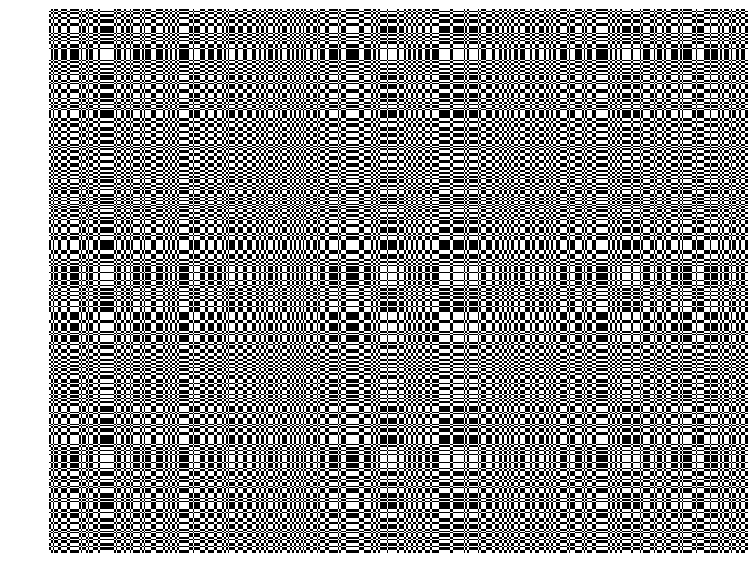
\includegraphics[height=3.3cm]{../img/KPP.pdf}}}
\newcommand{\kqq}{\mathord{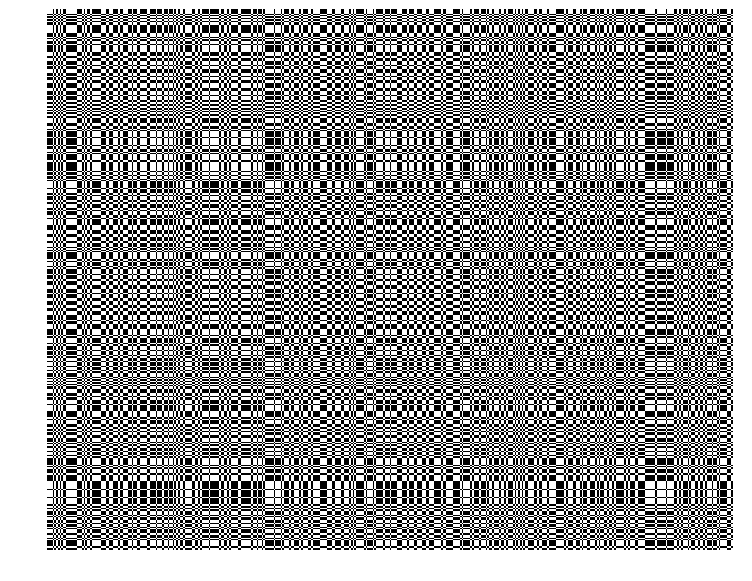
\includegraphics[height=3.3cm]{../img/KQQ.pdf}}}
\newcommand{\kpq}{\mathord{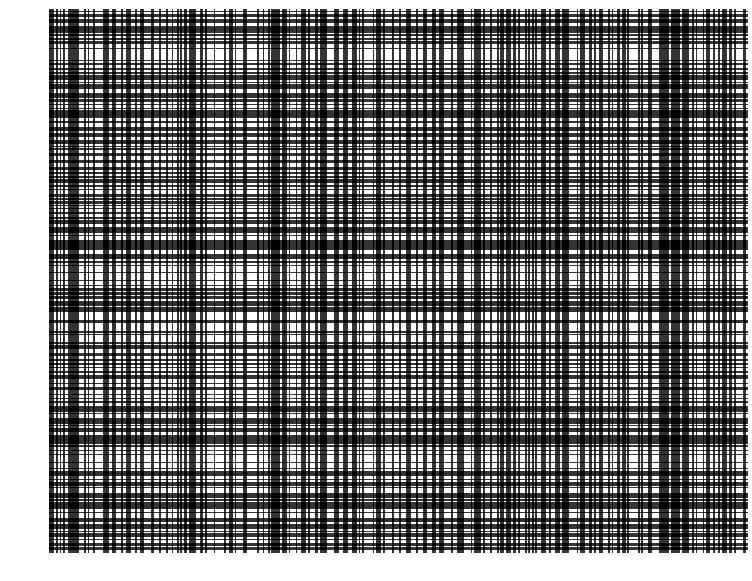
\includegraphics[height=3.3cm]{../img/KPQ.pdf}}}
\newcommand{\gram}{\mathord{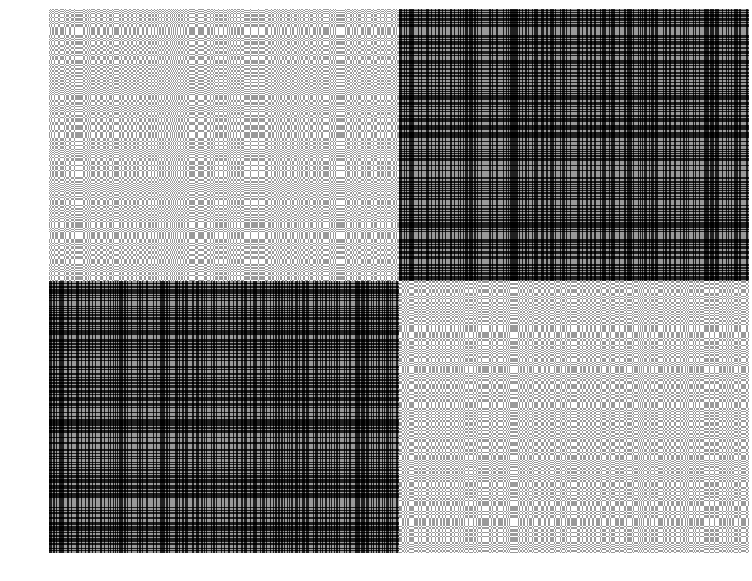
\includegraphics[height=4cm]{../img/Gram.pdf}}}
\newcommand{\gramn}{\mathord{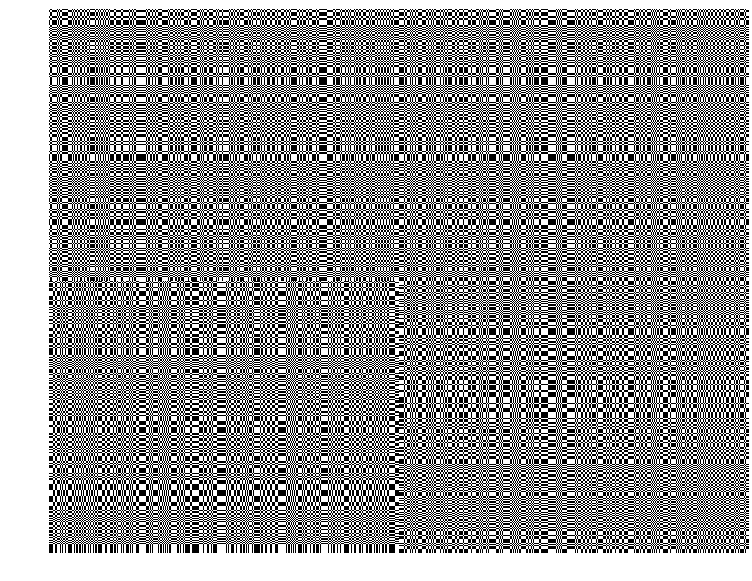
\includegraphics[height=4cm]{../img/Gramn.pdf}}}

\newcommand{\kppmem}{\mathord{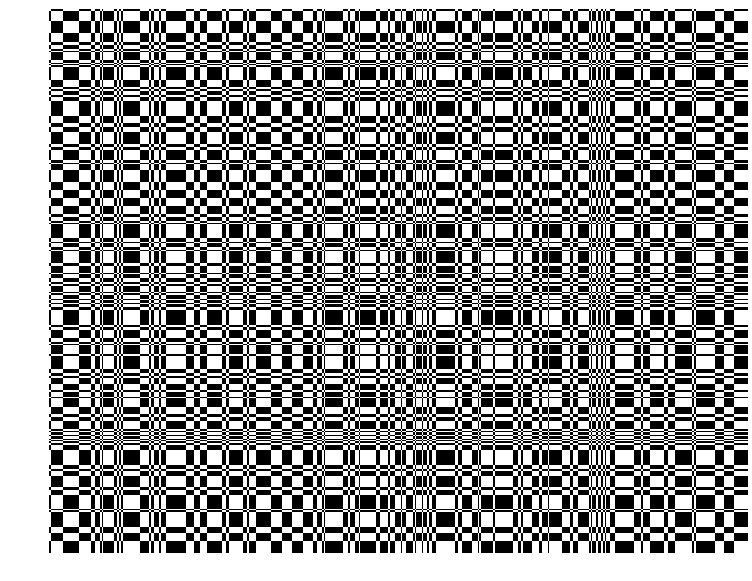
\includegraphics[height=3.3cm]{../img/KPPmem.pdf}}}
\newcommand{\kqqmem}{\mathord{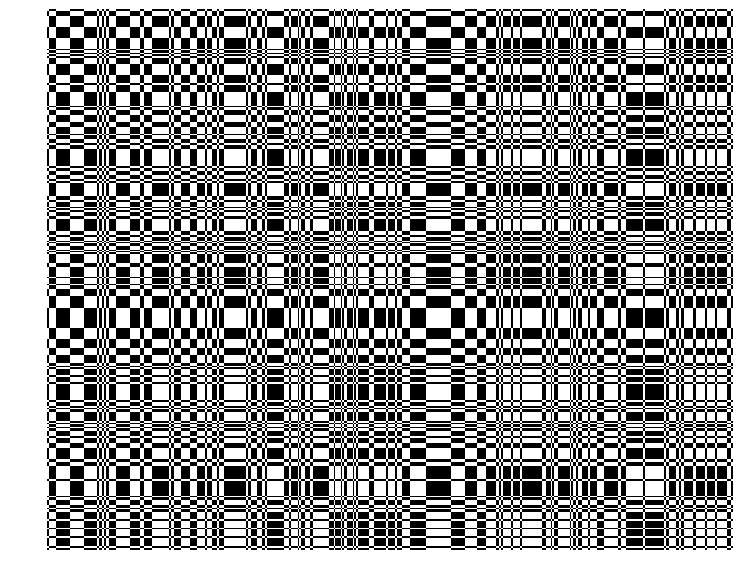
\includegraphics[height=3.3cm]{../img/KQQmem.pdf}}}
\newcommand{\kpqmem}{\mathord{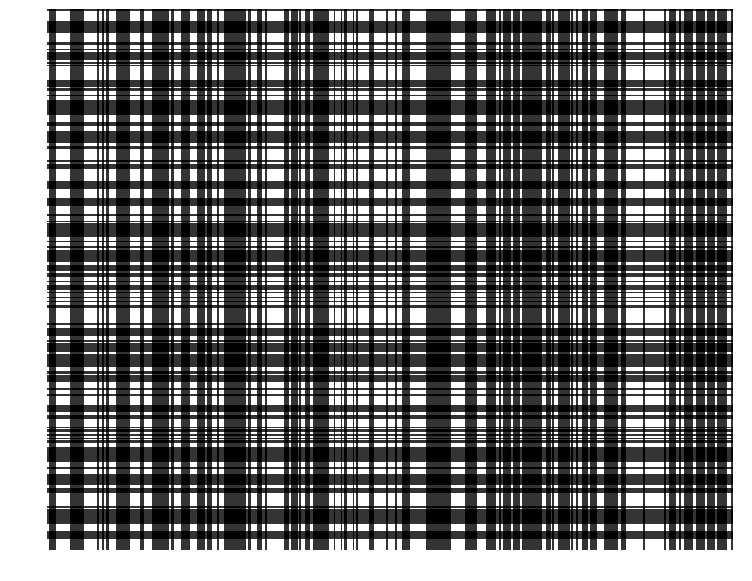
\includegraphics[height=3.3cm]{../img/KPQmem.pdf}}}
\newcommand{\grammem}{\mathord{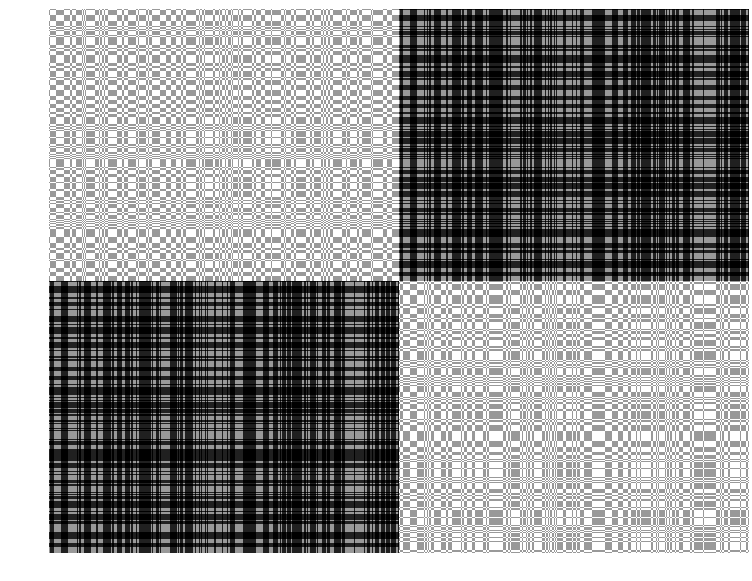
\includegraphics[height=4cm]{../img/Grammem.pdf}}}
\newcommand{\gramnmem}{\mathord{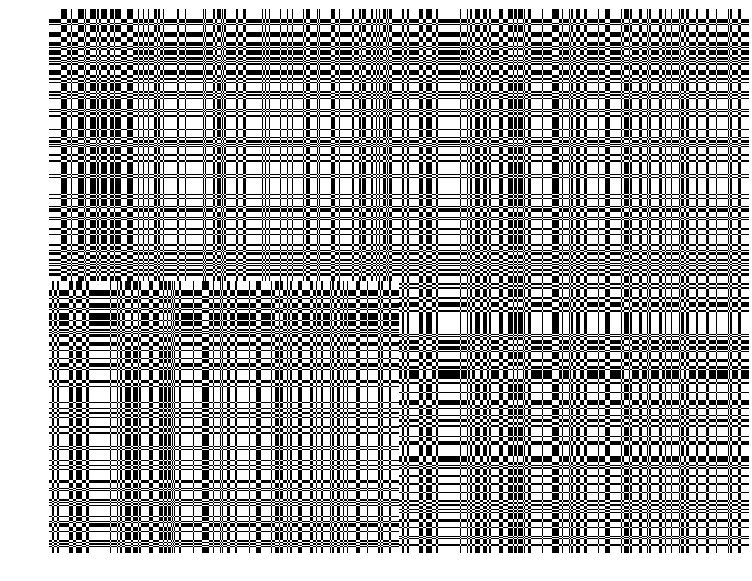
\includegraphics[height=4cm]{../img/Gramnmem.pdf}}}
\newcommand{\wildAlt}{\mathord{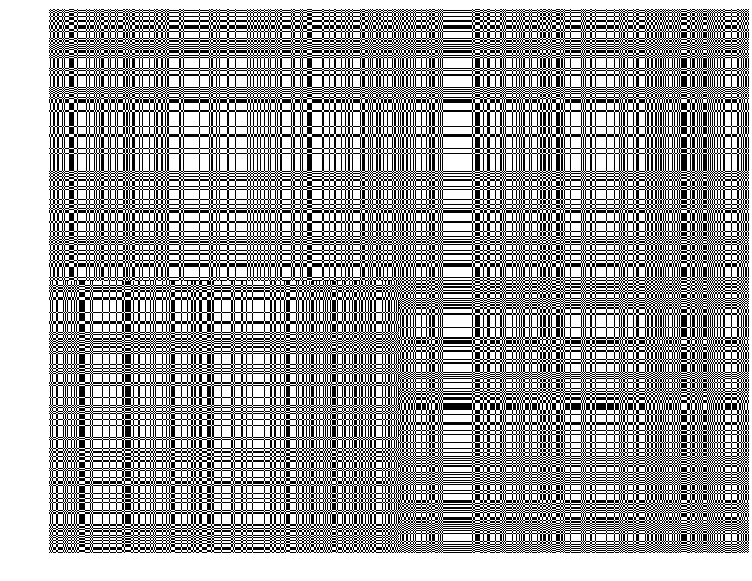
\includegraphics[height=4cm]{../img/wildAlt.pdf}}}
\newcommand{\wildNull}{\mathord{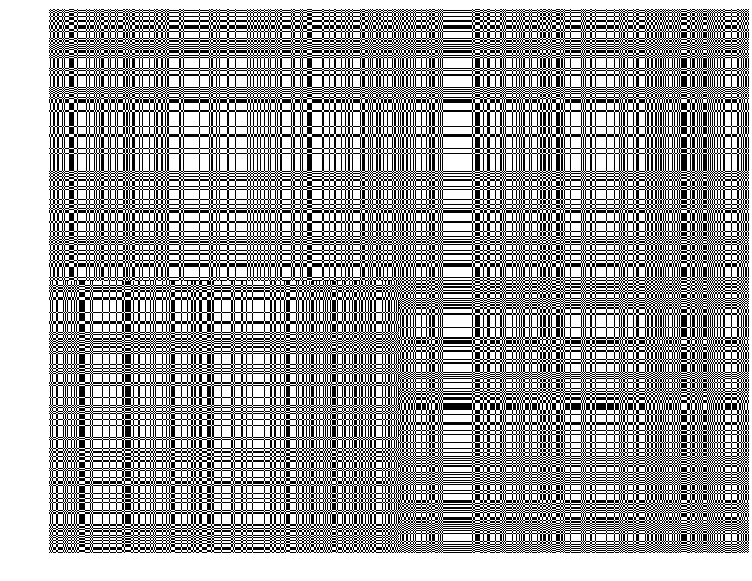
\includegraphics[height=4cm]{../img/wildNull.pdf}}}
\newcommand{\wildMatrix}{\mathord{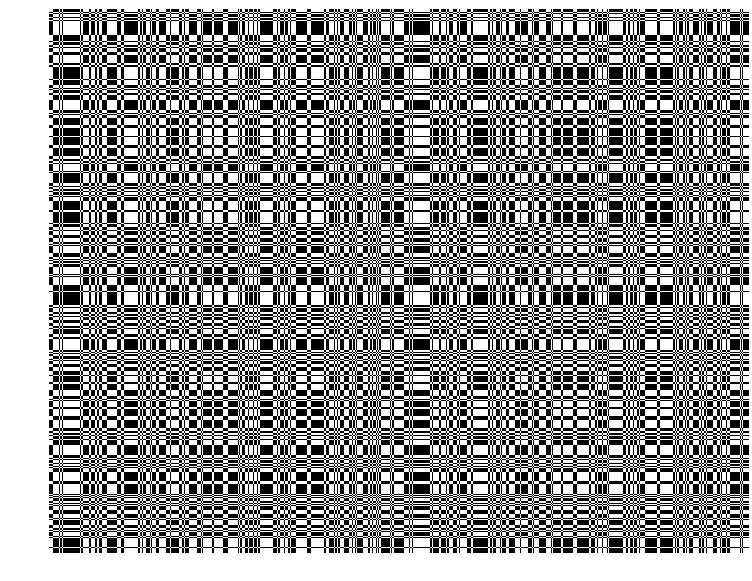
\includegraphics[height=3.3cm]{../img/wildmatrix.pdf}}}
% ------------------------------------------------------------
% first column: 
% ------------------------------------------------------------
% Attention: between the end of one column and the begin of the next
% column must not be spaces - otherwise latex thinks that it has to
% make a pagebreak... see below how I did it!


\begin{PosterColumn} % this creates a column, you have to care yourself
% that it doesn't get too long for the poster
%

% the old pbox command does not exist any more, as it hacked the ps
% file (which of course does not work any more with pdflatex). So
% please use this one instead: 
%
\PosterBox{  Is  $ \color{blue} P$ the same  distribution as $\color{red} Q$ ?}
\begin{minipage}[c]{0.5\textwidth}  
  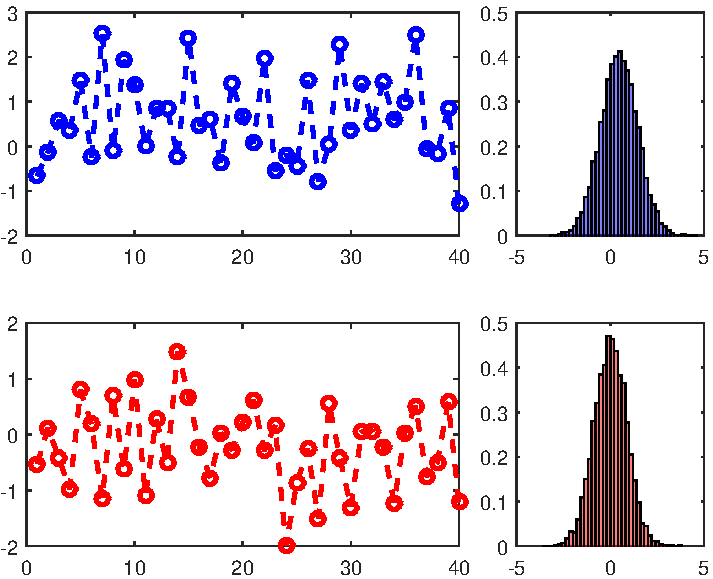
\includegraphics[width=\textwidth]{../img/introDep.pdf}
\end{minipage}
%
\begin{minipage}[c]{0.5\textwidth}
	
\textbf{Where one can use Maximum Mean Discrepancy ?}
\begin{itemize}[leftmargin=1in]	
	\item Markov chains diagnostics
	\item Change point detection
\end{itemize}
\textbf{ Other tests}
\begin{itemize}[leftmargin=1in]	
	\item Hilbert Schmidt Independence Criterion
		\begin{itemize}		
			\item Dependency structure in financial markets 
			\item Brain region activation
		\end{itemize}
	\item Three Variables Interaction 	
\end{itemize}
	
\end{minipage}   
%%%%%%%%%%%%%%%%


% ------------------------------------------------------------
\PosterBox{Background}
% ------------------------------------------------------------
\Blue{{\bf Similarity}}


\begin{minipage}[c]{0.5\textwidth}  
 \begin{align*}
K_{{\color{blue}P,P}}=
\begin{bmatrix}
	k( {\color{blue}X_1},{\color{blue}X_1)} &   \ldots & k({\color{blue}X_1},{\color{blue}X_n})\\
	\vdots &  \ddots & \vdots\\
	k({\color{blue}X_n},{\color{blue}X_1})  &  \ldots & k({\color{blue}X_n},{\color{blue}X_n})
\end{bmatrix} = 
\begin{matrix}
\kppmem
\end{matrix}
\\
K_{{\color{red}Q,Q}}=
\begin{bmatrix}
	k({\color{red}Y_1},{\color{red}Y_1)} &   \ldots & k({\color{red}Y_1},{\color{red}Y_n})\\
	\vdots &  \ddots & \vdots\\
	k({\color{red}Y_n},{\color{red}Y_1})  &  \ldots & k({\color{red}Y_n},{\color{red}Y_n})
\end{bmatrix}= 
\begin{matrix}
\kqqmem
\end{matrix}
\\
K_{{\color{blue}P,\color{red}Q}}=
\begin{bmatrix}
	k({\color{blue}X_1},{\color{red}Y_1}) &   \ldots & k({\color{blue}X_1},{\color{red}Y_n})\\
	\vdots &  \ddots & \vdots\\
	k({\color{blue}X_n},{\color{red}Y_1})  &  \ldots & k({\color{blue}X_n},{\color{red}Y_n})
\end{bmatrix}=
\begin{matrix}
\kpqmem
\end{matrix}
\end{align*}
\end{minipage}
\begin{minipage}[c]{0.5\textwidth}  
  \begin{align*}
{\color{blue} P} \neq {\color{red} Q} \Rightarrow
\begin{bmatrix}
	K_{\color{blue}P,P}  &   K_{{\color{blue}P,\color{red}Q}}\\
	K_{{\color{red}Q},{\color{blue}P}} &  K_{\color{red}Q,Q}
\end{bmatrix} = 
\begin{matrix}
\gram
\end{matrix}
\end{align*}
\begin{align*}
{\color{blue} P }= {\color{red} Q} \Rightarrow
\begin{bmatrix}
	K_{\color{blue}P,P}  &   K_{{\color{blue}P,\color{red}Q}}\\
	K_{{\color{red}Q},{\color{blue}P}} &  K_{\color{red}Q,Q}
\end{bmatrix} = 
\begin{matrix}
\gramn
\end{matrix}
\end{align*}
\end{minipage}\\

\Blue{{\bf Quantifying Similarity}}


\begin{minipage}[c]{0.4\textwidth}
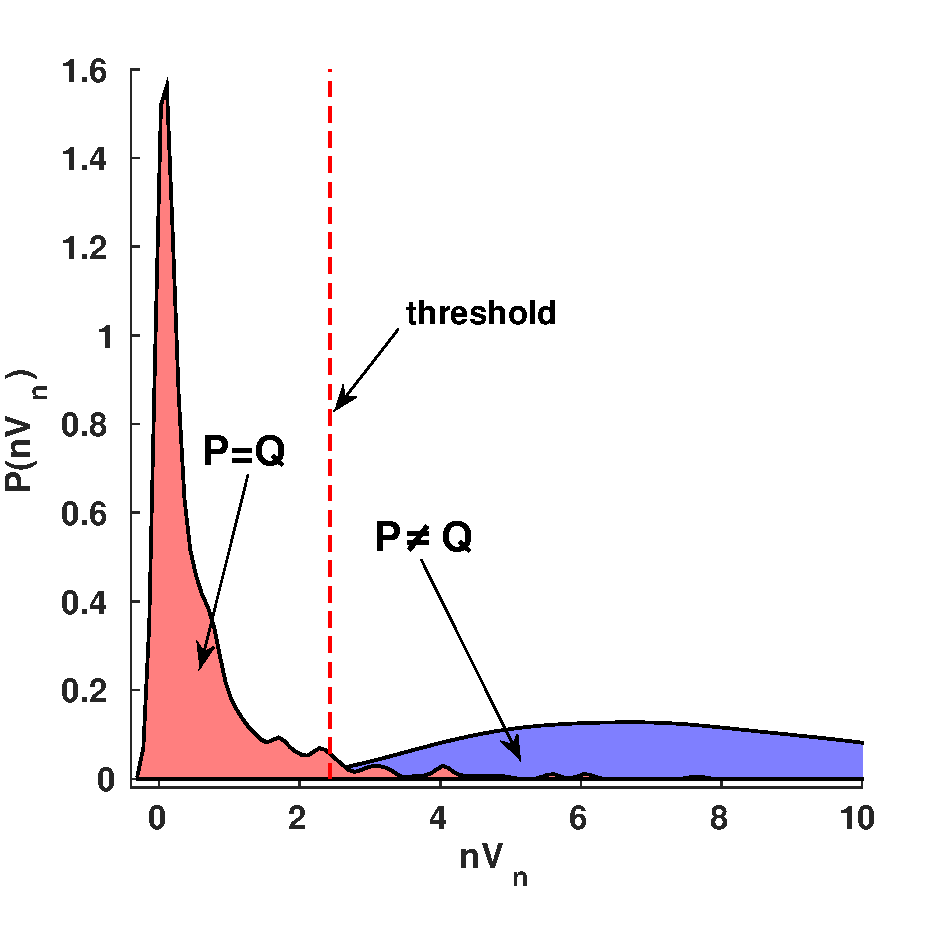
\includegraphics[width=\textwidth]{../img/altAndNull.pdf}
\end{minipage}
\begin{minipage}[c]{0.59\textwidth}
The $V$-statistics quantifies the concept of similarity.  
\begin{align*}
 \color{mpigreen} V_n = \overline{ K_{\color{blue}P,P}} + \overline{ K_{\color{red}Q,Q} } - 2 \overline{  K_{{\color{blue}P,\color{red}Q}} }.
\end{align*}
Explicitly 
\begin{align*}
 V_n = \frac{1}{n^2} \sum_{1 \leq i,j \leq n} k(X_i,X_j) + k(Y_i,Y_j) - k(X_i,Y_j) - k(X_j,Y_i).
\end{align*}
The degeneracy: if $ {\color{blue} P}= \color{red} Q$, then for $i \neq j$ 
\begin{align*}
 \ev \left[ k(X_i,X_j) + k(Y_i,Y_j) - k(X_i,Y_j) - k(X_j,Y_i) \right]=0 .
\end{align*}
\end{minipage}\\


\Blue{{\bf Estimation of $V_n$ via Permutation}}


\begin{minipage}[c]{0.59\textwidth}
$$W= (-1,1,1,\quad \cdots \quad,-1,-1,-1)$$
\begin{align*}
&{\begin{bmatrix}
	K_{\color{blue}P,P}  &   K_{{\color{blue}P,\color{red}Q}}\\
	K_{{\color{red}Q},{\color{blue}P}} &  K_{\color{red}Q,Q}
\end{bmatrix} } & \odot
&\begin{bmatrix}
\Scale[2] {W \trans{W}}
\end{bmatrix} &= 
&\begin{bmatrix}
\Scale[2] ?
\end{bmatrix} \\
&\begin{matrix}
\gram
\end{matrix} &\odot
&\begin{matrix}
\kpp
\end{matrix} &=
&\begin{matrix} 
\gramn
\end{matrix} \\
&\begin{matrix}
\gramn
\end{matrix} &\odot
&\begin{matrix}
\kpp
\end{matrix} &=
&\begin{matrix} 
\gramn
\end{matrix} \\
\end{align*}

\end{minipage}
\begin{minipage}[c]{0.4\textwidth}
\begin{align*}
 \color{mpigreen} V_{n,p} = \overline{ {\begin{bmatrix}
	K_{\color{blue}P,P}  &   K_{{\color{blue}P,\color{red}Q}}\\
	K_{{\color{red}Q},{\color{blue}P}} &  K_{\color{red}Q,Q}
\end{bmatrix} }  \odot
\begin{bmatrix}
\Scale[2] {W \trans{W}}
\end{bmatrix}}
\end{align*}

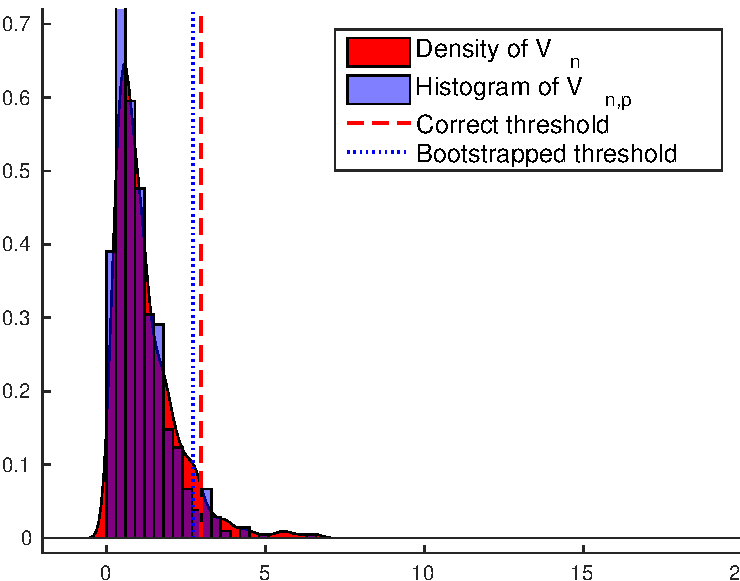
\includegraphics[width=\textwidth]{../img/permfail_ecdf1.pdf}

\end{minipage}





\end{PosterColumn}
%%
%% ------------------------------------------------------------
%% second column: 
%% ------------------------------------------------------------
%%
\begin{PosterColumn}



\PosterBox{Permutation Tests for Random Processes}


\Blue{{\bf Memory of the Processes}}

\begin{minipage}[c]{0.4\textwidth}
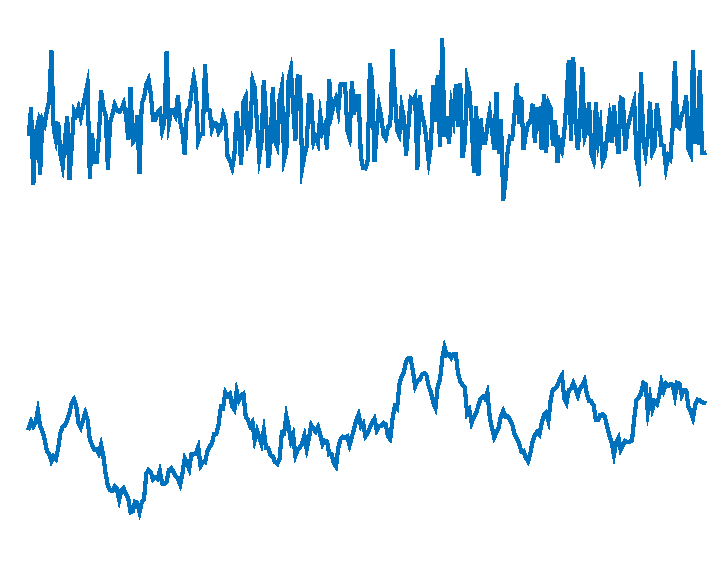
\includegraphics[width=\textwidth]{../img/processes.pdf}
\end{minipage}
\begin{minipage}[c]{0.5\textwidth}
{\larger[2]$$Q_t =  \mathbf{ \color{red} 0.14} Q_{t-1} + 0.98\epsilon_t$$ }
    Processes with different memory 
	{\larger[2]$$Z_t=   \mathbf{ \color{red} 0.97} Z_{t-1} +  0.22\epsilon_t.$$ }	
\end{minipage}



\Blue{{\bf Estimation of $V_n$ via Permutation Fails}}

\vspace{1cm}

\begin{minipage}[c]{0.24\textwidth}
$$\text{Memory } 0.1$$
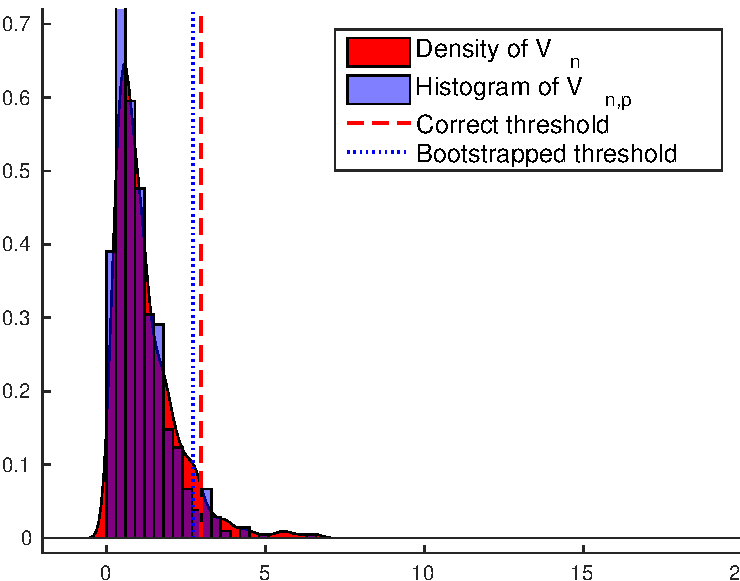
\includegraphics[width=\textwidth]{../img/permfail_ecdf1.pdf} 
\end{minipage}
\begin{minipage}[c]{0.24\textwidth}
$$\text{Memory }0.2$$
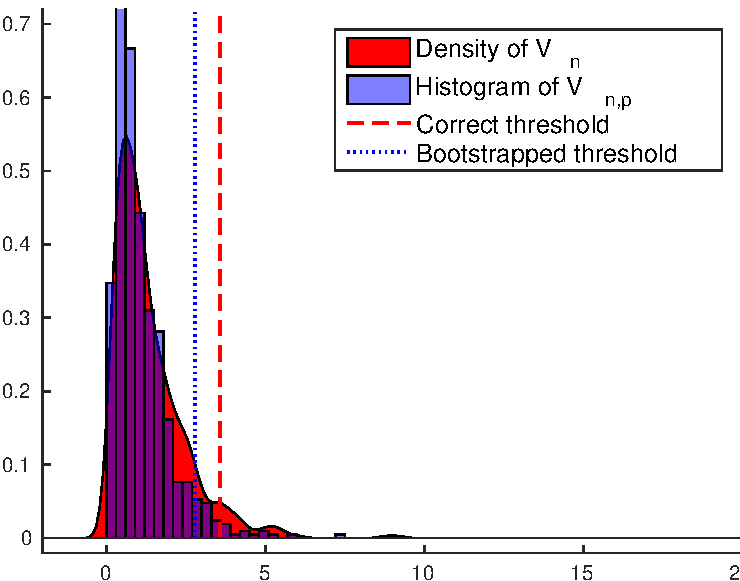
\includegraphics[width=\textwidth]{../img/permfail_ecdf2.pdf} 
\end{minipage}
\begin{minipage}[c]{0.24\textwidth}
$$\text{Memory }0.3$$
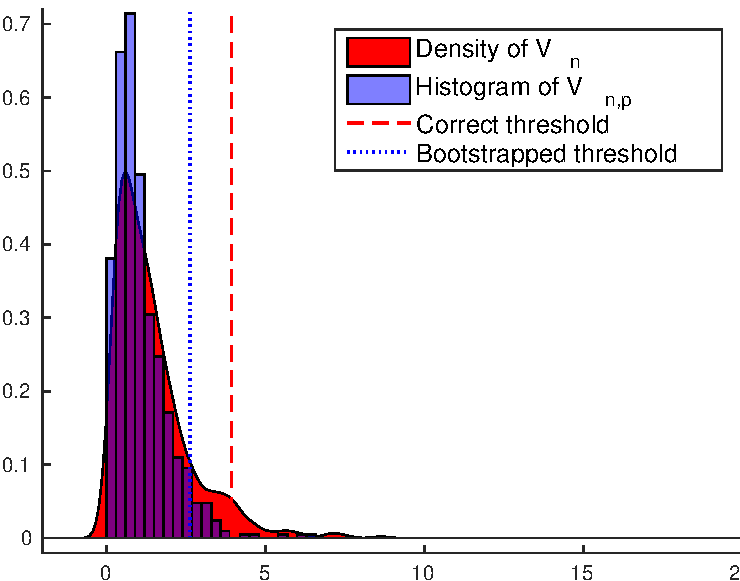
\includegraphics[width=\textwidth]{../img/permfail_ecdf3.pdf} 
\end{minipage}
\begin{minipage}[c]{0.24\textwidth}
$$\text{Memory }0.4$$
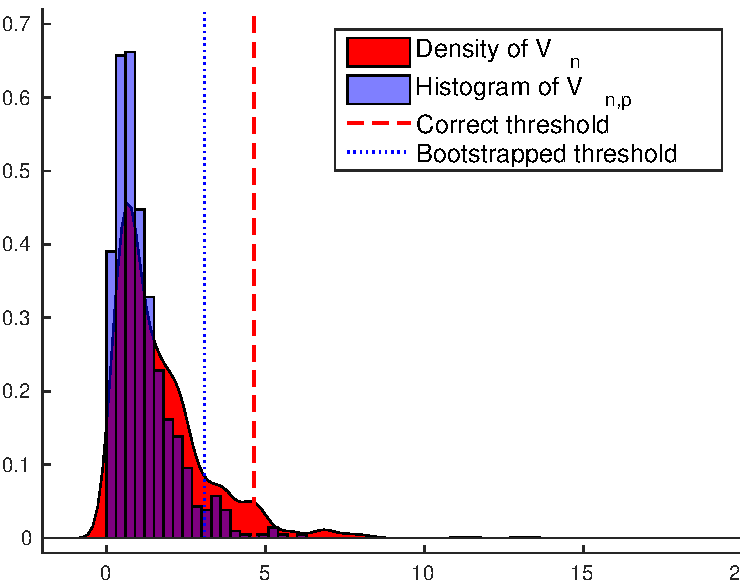
\includegraphics[width=\textwidth]{../img/permfail_ecdf4.pdf} 
\end{minipage}

\begin{minipage}[c]{0.24\textwidth}
$$\text{Memory }0.5$$
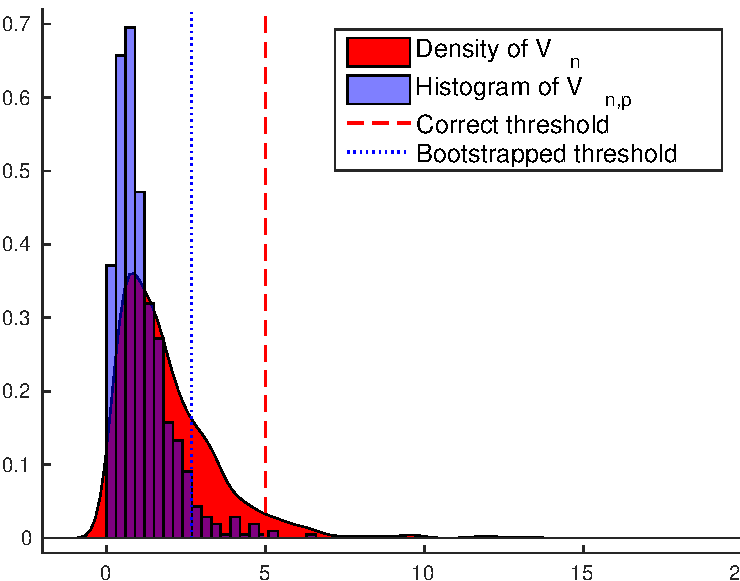
\includegraphics[width=\textwidth]{../img/permfail_ecdf5.pdf} 
\end{minipage}
\begin{minipage}[c]{0.24\textwidth}
$$\text{Memory }0.6$$
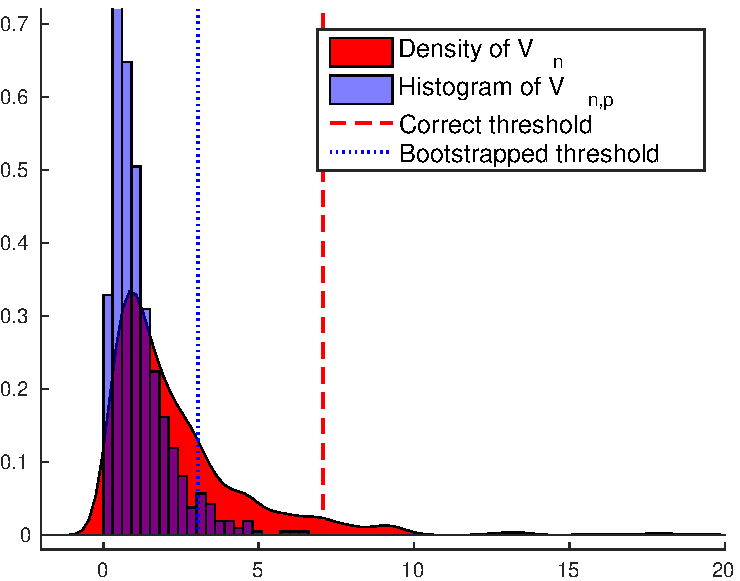
\includegraphics[width=\textwidth]{../img/permfail_ecdf6.pdf} 
\end{minipage}
\begin{minipage}[c]{0.24\textwidth}
$$\text{Memory }0.7$$
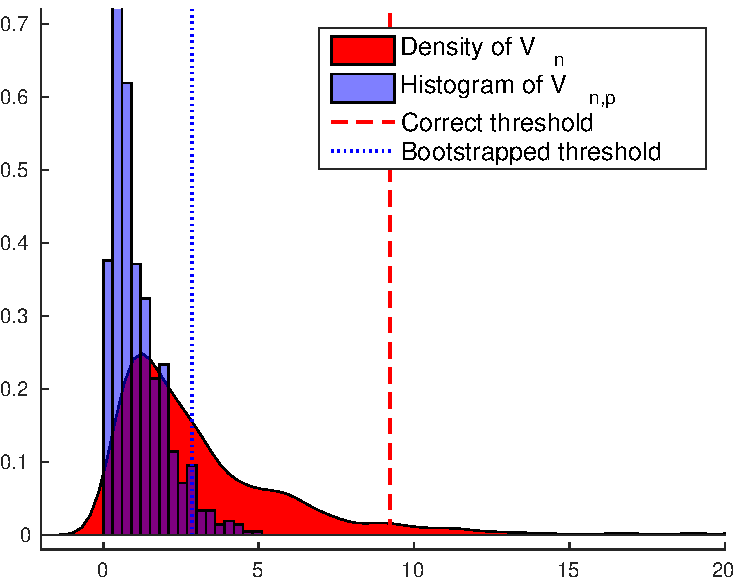
\includegraphics[width=\textwidth]{../img/permfail_ecdf7.pdf} 
\end{minipage}
\begin{minipage}[c]{0.24\textwidth}
$$\text{Memory }0.8$$
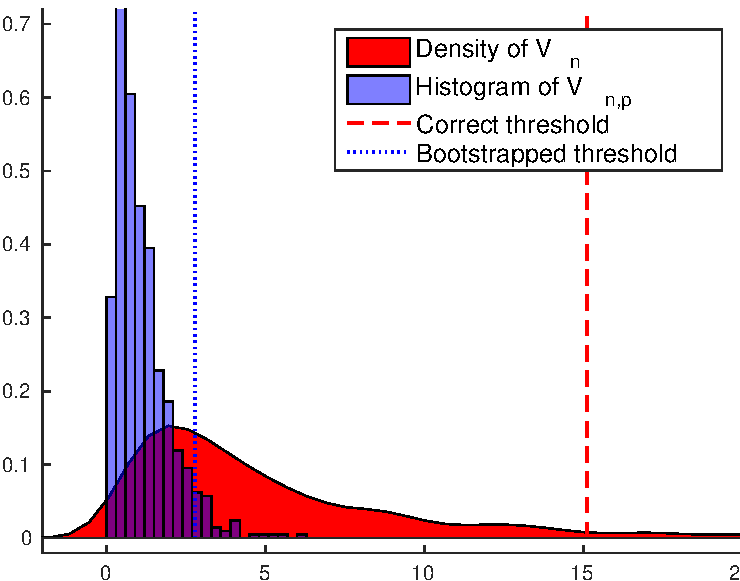
\includegraphics[width=\textwidth]{../img/permfail_ecdf8.pdf} 
\end{minipage}

\vspace{1cm}

\Blue{{\bf The Reason why Permutation Test Fails }}

\begin{minipage}[c]{0.49\textwidth}
\begin{align*}
\Scale[1.52]{W= (-1,1\cdots,-1,-1,-1)}
\end{align*}
\begin{align*}
&{\begin{bmatrix}
	K_{\color{blue}P,P}  &   K_{{\color{blue}P,\color{red}Q}}\\
	K_{{\color{red}Q},{\color{blue}P}} &  K_{\color{red}Q,Q}
\end{bmatrix} } & \odot
&\begin{bmatrix}
\Scale[2] {W \trans{W}}
\end{bmatrix} &= 
&\begin{bmatrix}
\Scale[2] ?
\end{bmatrix} \\
\end{align*}

\end{minipage}
\begin{minipage}[c]{0.49\textwidth}
\begin{align*}
&\begin{matrix}
\grammem
\end{matrix} &\odot
&\begin{matrix}
\kpp
\end{matrix} &=
&\begin{matrix} 
\gramn
\end{matrix} \\
&\begin{matrix}
\gramnmem
\end{matrix} &\odot
&\begin{matrix}
\kpp
\end{matrix} &=
&\begin{matrix} 
\gramn
\end{matrix} \\
\end{align*}

\end{minipage}
\PosterBox{Wild Bootstrap for Random Processes}

\begin{minipage}[c]{0.49\textwidth}
\begin{center}
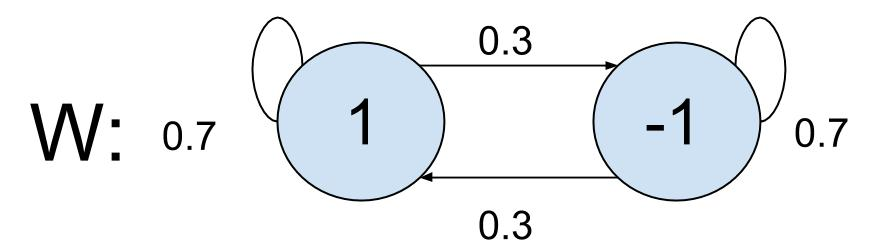
\includegraphics[height=3.5cm]{../img/markowChain.jpg}
\end{center}

\begin{align*}
&{\begin{bmatrix}
	K_{\color{blue}P,P}  &   K_{{\color{blue}P,\color{red}Q}}\\
	K_{{\color{red}Q},{\color{blue}P}} &  K_{\color{red}Q,Q}
\end{bmatrix} } & \odot
&{\begin{bmatrix}
	W\trans{W}  &  -W\trans{W}\\
	-W\trans{W}  &  W\trans{W}
\end{bmatrix} }&= 
&\begin{bmatrix}
\Scale[2] ?
\end{bmatrix} \\
\end{align*}

\end{minipage}
\begin{minipage}[c]{0.49\textwidth}
\begin{align*}
&\begin{matrix}
\grammem
\end{matrix} &\odot
&\begin{matrix}
\wildMatrix
\end{matrix} &=
&\begin{matrix} 
\wildAlt
\end{matrix} \\
&\begin{matrix}
\gramnmem
\end{matrix} &\odot
&\begin{matrix}
\wildMatrix
\end{matrix} &=
&\begin{matrix} 
\wildNull
\end{matrix} \\
\end{align*}

\end{minipage}


\Blue{{\bf Estimation of $V_n$ via Wild Bootstrap}}

\begin{align*}
\Scale[1.5]{  \color{mpigreen} V_{n,w}=\overline{
\begin{bmatrix}
	K_{\color{blue}P,P}  &   K_{{\color{blue}P,\color{red}Q}}\\
	K_{{\color{red}Q},{\color{blue}P}} &  K_{\color{red}Q,Q}
\end{bmatrix}   \odot
\begin{bmatrix}
	W\trans{W}  &  -W\trans{W}\\
	-W\trans{W}  &  W\trans{W}
\end{bmatrix} }}
\end{align*}


\end{PosterColumn}
%%
\begin{PosterColumn}


\Blue{{\bf Estimation of $V_n$ via Permutation}}

\begin{minipage}[c]{0.24\textwidth} $$\text{Memory } 0.1$$
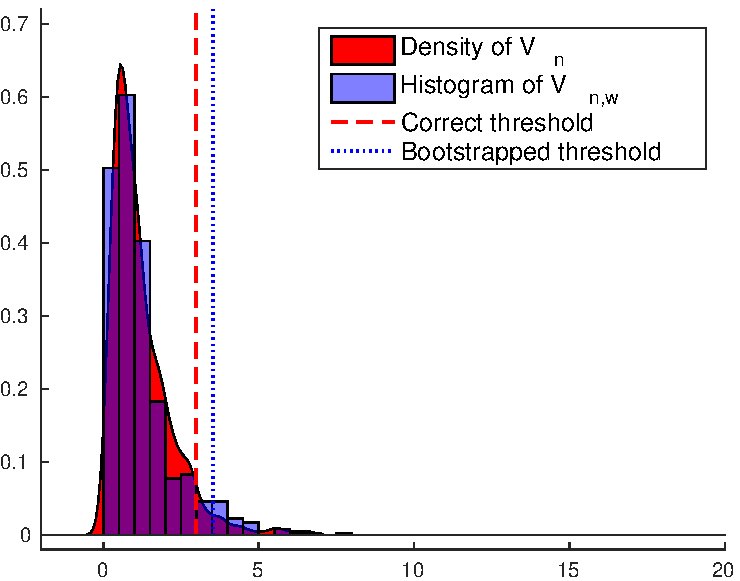
\includegraphics[width=\textwidth]{../img/wild_ecdf1.pdf} 
\end{minipage}
\begin{minipage}[c]{0.24\textwidth} $$\text{Memory } 0.2$$
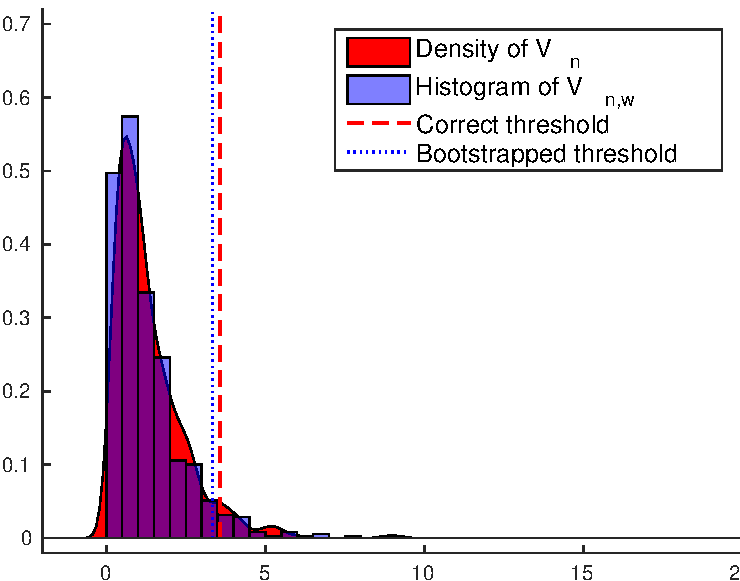
\includegraphics[width=\textwidth]{../img/wild_ecdf2.pdf} 
\end{minipage}
\begin{minipage}[c]{0.24\textwidth} $$\text{Memory } 0.3$$
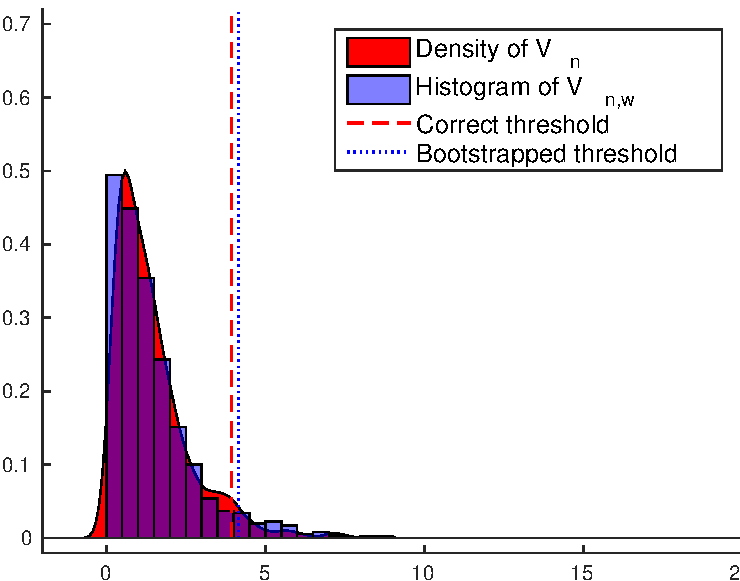
\includegraphics[width=\textwidth]{../img/wild_ecdf3.pdf} 
\end{minipage}
\begin{minipage}[c]{0.24\textwidth} $$\text{Memory } 0.4$$
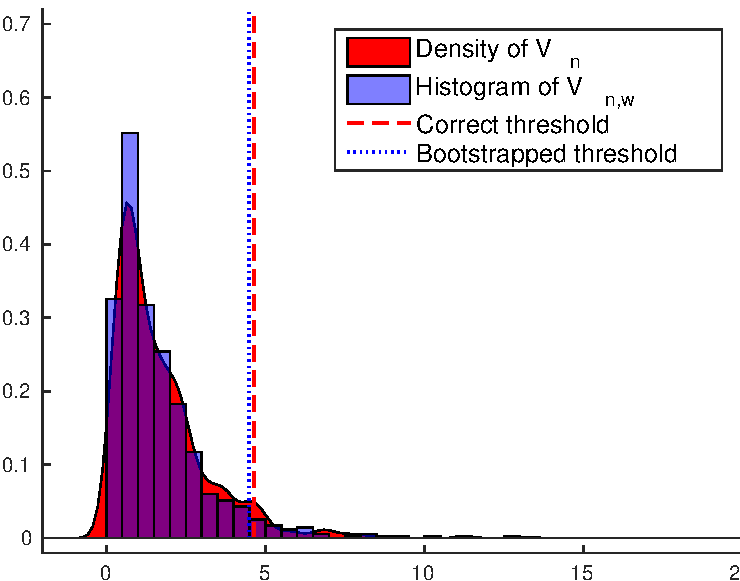
\includegraphics[width=\textwidth]{../img/wild_ecdf4.pdf} 
\end{minipage}

\begin{minipage}[c]{0.24\textwidth} $$\text{Memory } 0.5$$
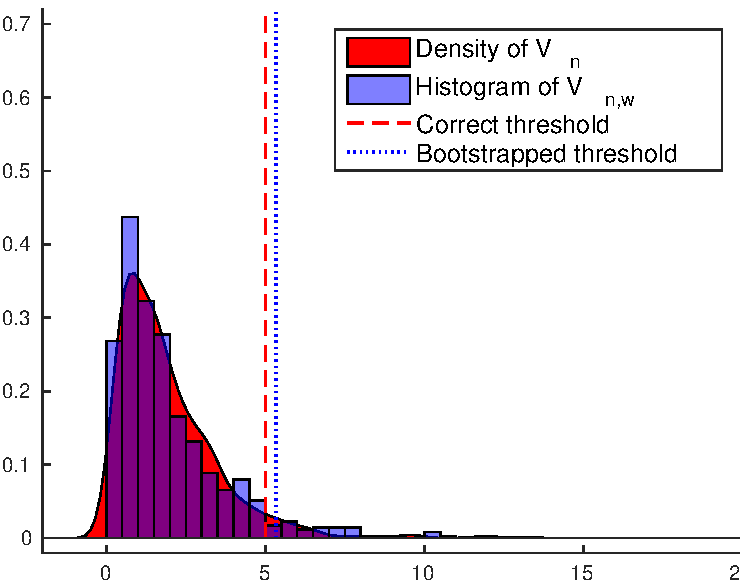
\includegraphics[width=\textwidth]{../img/wild_ecdf5.pdf} 
\end{minipage}
\begin{minipage}[c]{0.24\textwidth} $$\text{Memory } 0.6$$
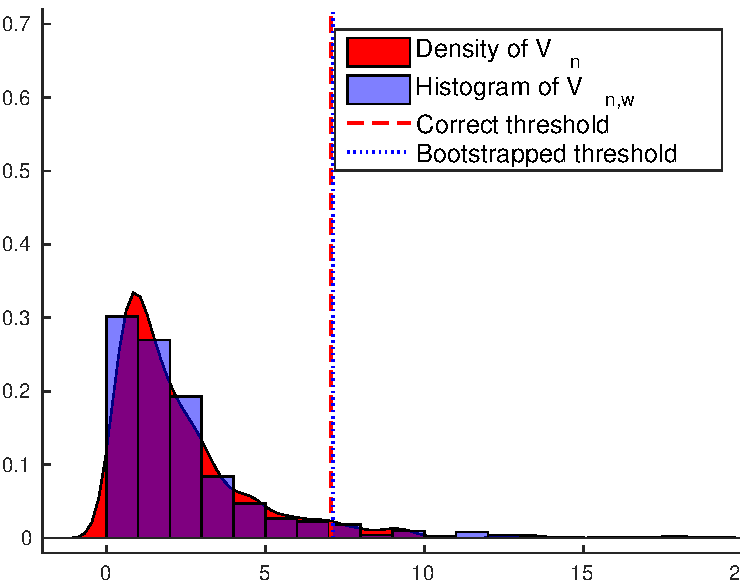
\includegraphics[width=\textwidth]{../img/wild_ecdf6.pdf} 
\end{minipage}
\begin{minipage}[c]{0.24\textwidth} $$\text{Memory } 0.7$$
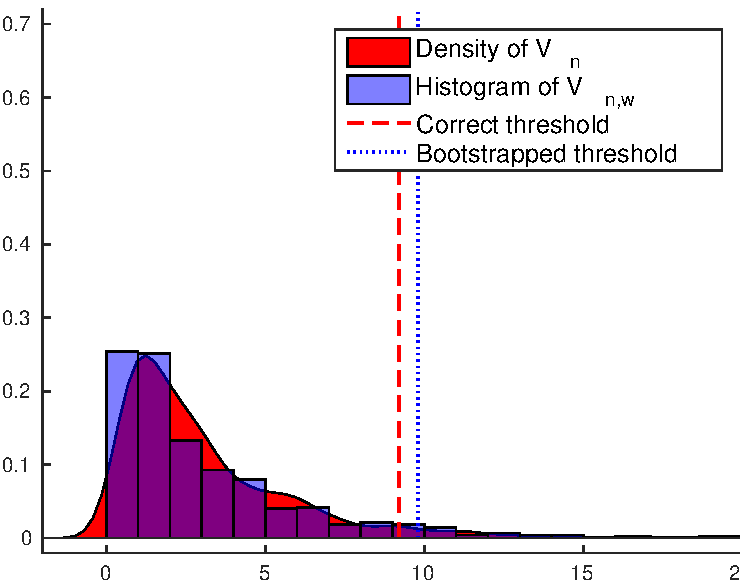
\includegraphics[width=\textwidth]{../img/wild_ecdf7.pdf} 
\end{minipage}
\begin{minipage}[c]{0.24\textwidth} $$\text{Memory } 0.8$$
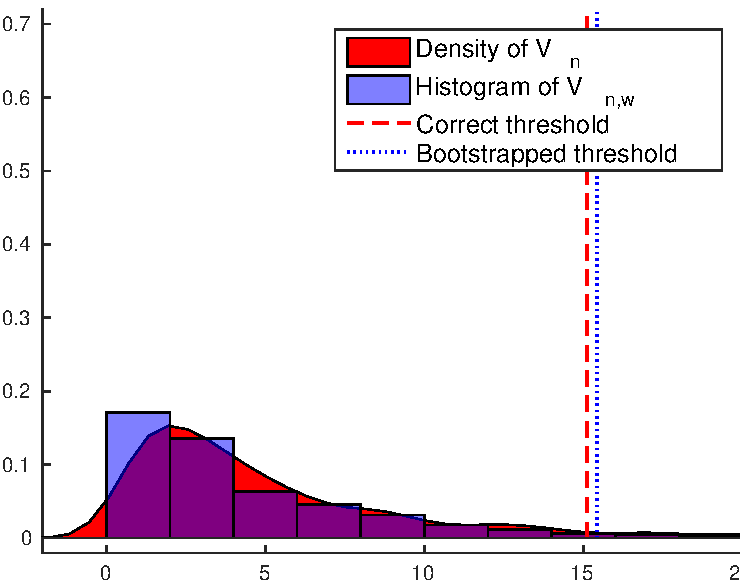
\includegraphics[width=\textwidth]{../img/wild_ecdf8.pdf} 
\end{minipage}

\vspace{1cm}
\PosterBox{Experiments}


\begin{minipage}[c]{0.4\textwidth}
\bf MCMC M.D.
\end{minipage}
\begin{minipage}[c]{0.6\textwidth}
\bf Indie Pop Group Predicts the Volume of the Dow Jones!
\end{minipage}


\begin{minipage}[c]{0.4\textwidth}
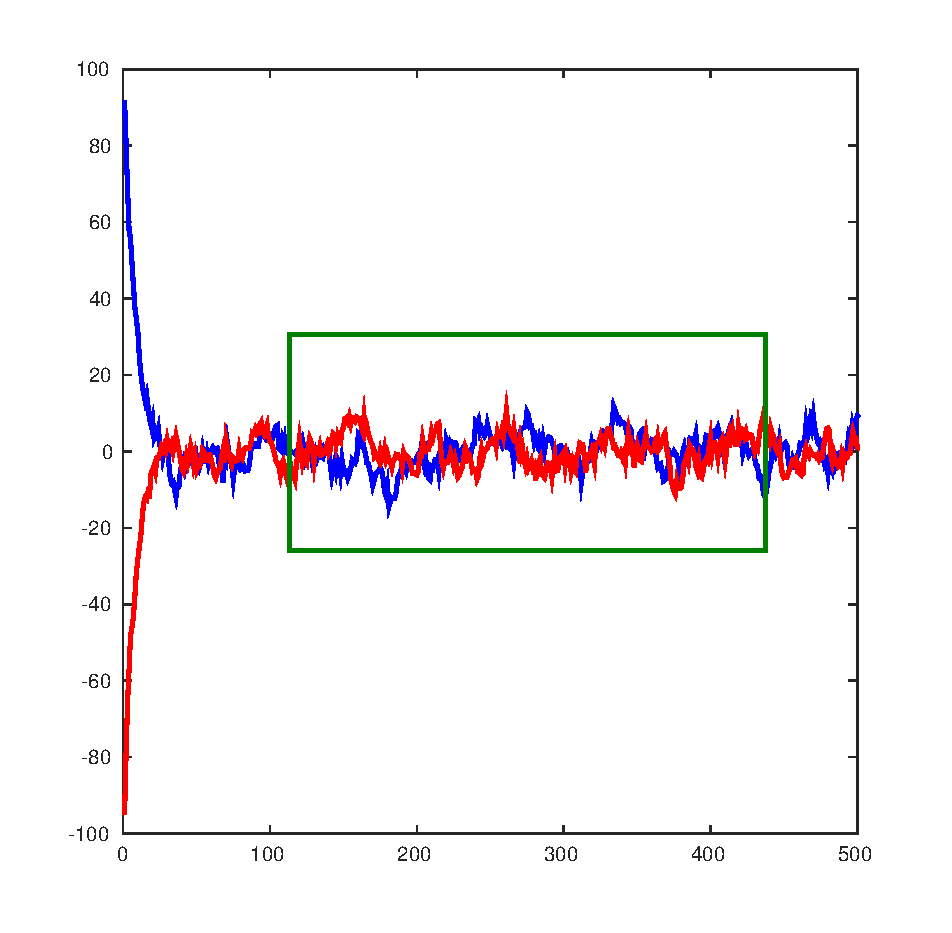
\includegraphics[width=\textwidth]{../img/mcmc.pdf}

\begin{center}
\begin{tabular}{ l | c  }
  \hline                       
  Test - MMD  &  Samples are different   \\  
    \hline   
  Permutation  & 68 \%   \\
    \hline   
  Wild Bootstrap    & 6 \%   \\
  \hline  
\end{tabular}
\end{center}
\end{minipage}
\begin{minipage}[c]{0.6\textwidth}
\vspace{3.3cm}
\begin{minipage}[c]{0.45\textwidth}
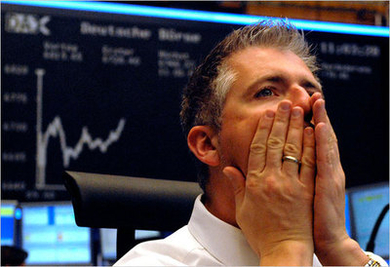
\includegraphics[width=\textwidth]{../img/sad-guys-on-trading-floors.jpg}
\end{minipage}  
\begin{minipage}[c]{0.45\textwidth}
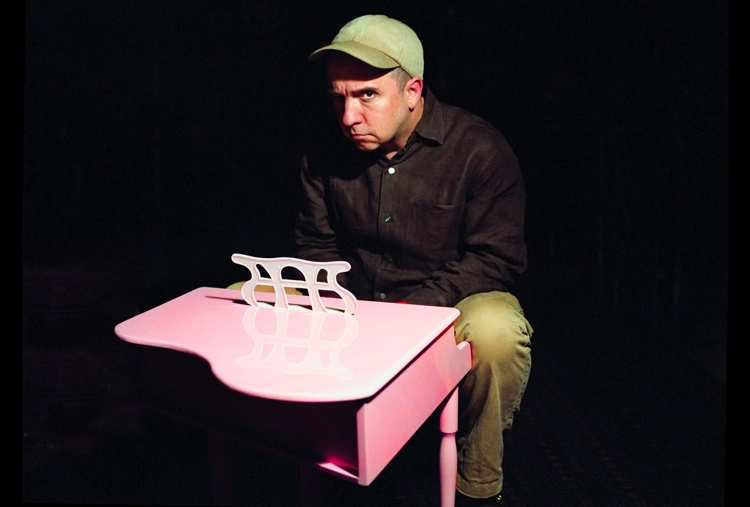
\includegraphics[width=\textwidth]{../img/strange_powers_01.jpg} 
\end{minipage} 
\begin{center}
\vspace{4cm}
\begin{tabular}{ l | c | c| c }
  \hline                       
  Test                   & p-value& Dependent   \\  
    \hline   
  Permutation HSIC       & 0.003  & Yes ! \\
    \hline   
  Wild Bootstrap HSIC    & 0.231  & \colorbox{red}{No} \\
  \hline  
\end{tabular}
\end{center}
\end{minipage}

\vspace{1cm}

\begin{minipage}[c]{0.6\textwidth}
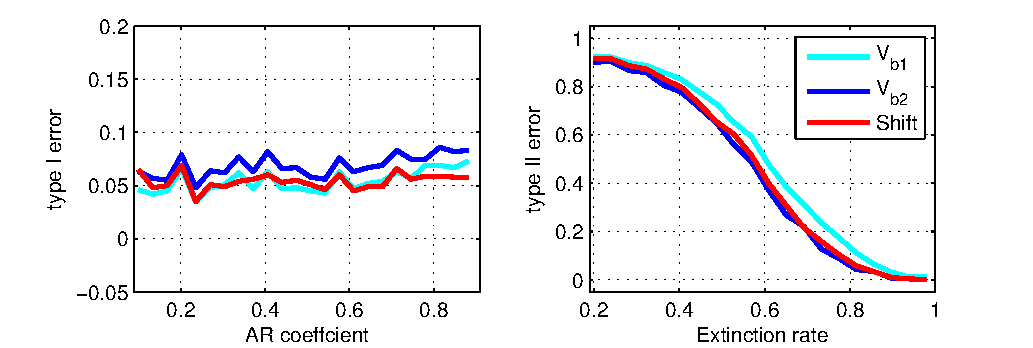
\includegraphics[width=\textwidth]{../img/arExtinct.pdf} 
\end{minipage}
\begin{minipage}[c]{0.4\textwidth}
Comparison of Shift-HSIC \cite{chwialkowski2014kernel}  and tests based on the wild bootstrap. The left panel shows the performance under the null hypothesis, where a larger AR coefficient implies a stronger temporal dependence. The right panel show the performance under the alternative hypothesis, where a larger extinction rate implies a greater dependence between processes.
\end{minipage}



\begin{minipage}[c]{0.4\textwidth}
The Kernel Cross-Spectral Density  \cite{besserve_statistical_2013} test is, to our knowledge, the only test procedure to reject the null hypothesis if there exist $t$,$t'$ such that $X_t$ and $Y_{t'}$ are dependent. In the experiments, we compare lag-HSIC with KCSD on two kinds of processes: one  inspired by econometrics and one from \cite{besserve_statistical_2013}. In both panels Type II error is plotted.
\end{minipage}
\begin{minipage}[c]{0.6\textwidth}
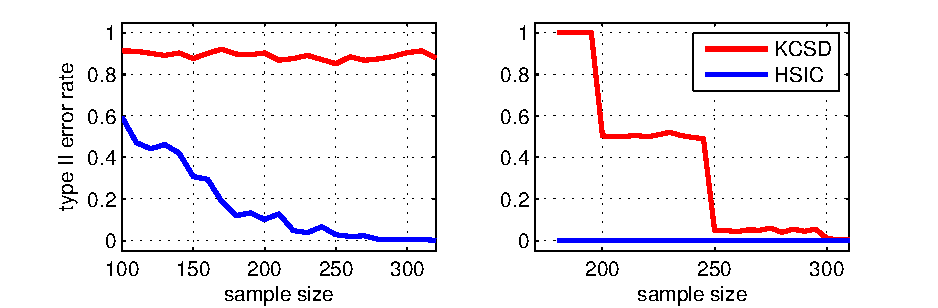
\includegraphics[width=\textwidth]{../img/varAndPhase.pdf} 
\end{minipage}

\small
\bibliographystyle{plain}
\bibliography{nips14Bib}


\end{PosterColumn}

\end{poster}
\end{document}

